\section{Introduction}
A social network is a graph of individuals and their interactions. It is a great resource to keep upto date what an individual's friends are upto. With the ever increasing use of web, social media is also used as an advertising tool. They are proved quite effective~\cite{F1969},~\cite{JP1987},~\cite{PM2001} to gain quick popularity by publicizing on popular social media sites like Facebook, MySpace, BlogSphere etc. than traditional advertising means. Their effectiveness is mainly due to high usage and size of users using it. Facebook for example has around 1.59 billion active users monthly~\footnote{http://www.statista.com/statistics/264810/number-of-monthly-active-facebook-users-worldwide/}. Another popular micro-blogging site called twitter has about 310 million monthly active users~\footnote{http://www.statista.com/statistics/282087/number-of-monthly-active-twitter-users/}. With such massive networks generating lot of data, everyone is constantly looking into ways of integrating the knowledge from them to make their systems more personal for their end users. Microsoft now ranks results, in its BING search, for a user using the search history from his/her social network~\cite{M2011}. There are also works on how probable a user performs an action given his/her friend committed the same action before~\cite{DJE2003}. The natural problem of social influence would be, `given a social network, how can we detect the players through which we can spread, or “diffuse”, the new technology in the most effective way`~\cite{EA2007}. Spread maximizing problem which try to find a minimal set S in a graph to gain maximum spread in a network is well studied in~\cite{MP2002}.

At the other end of the spectrum are the spatial networks. With the ever increasing number of wearables everyday like Jawbone, Fitbit, smart watches (pebble, apple watch) there is an abundance of data in this realm too. Importantly with the rapid increase in the number of mobile phone users, this data is already being tied to Social Network data and the two realms are coming together. Popular social network sites like Facebook have a number of features which prompt users to add spatial information like check-ins, traveling posts, geotagged photos etc.

\begin{figure}[t]
	\centering
	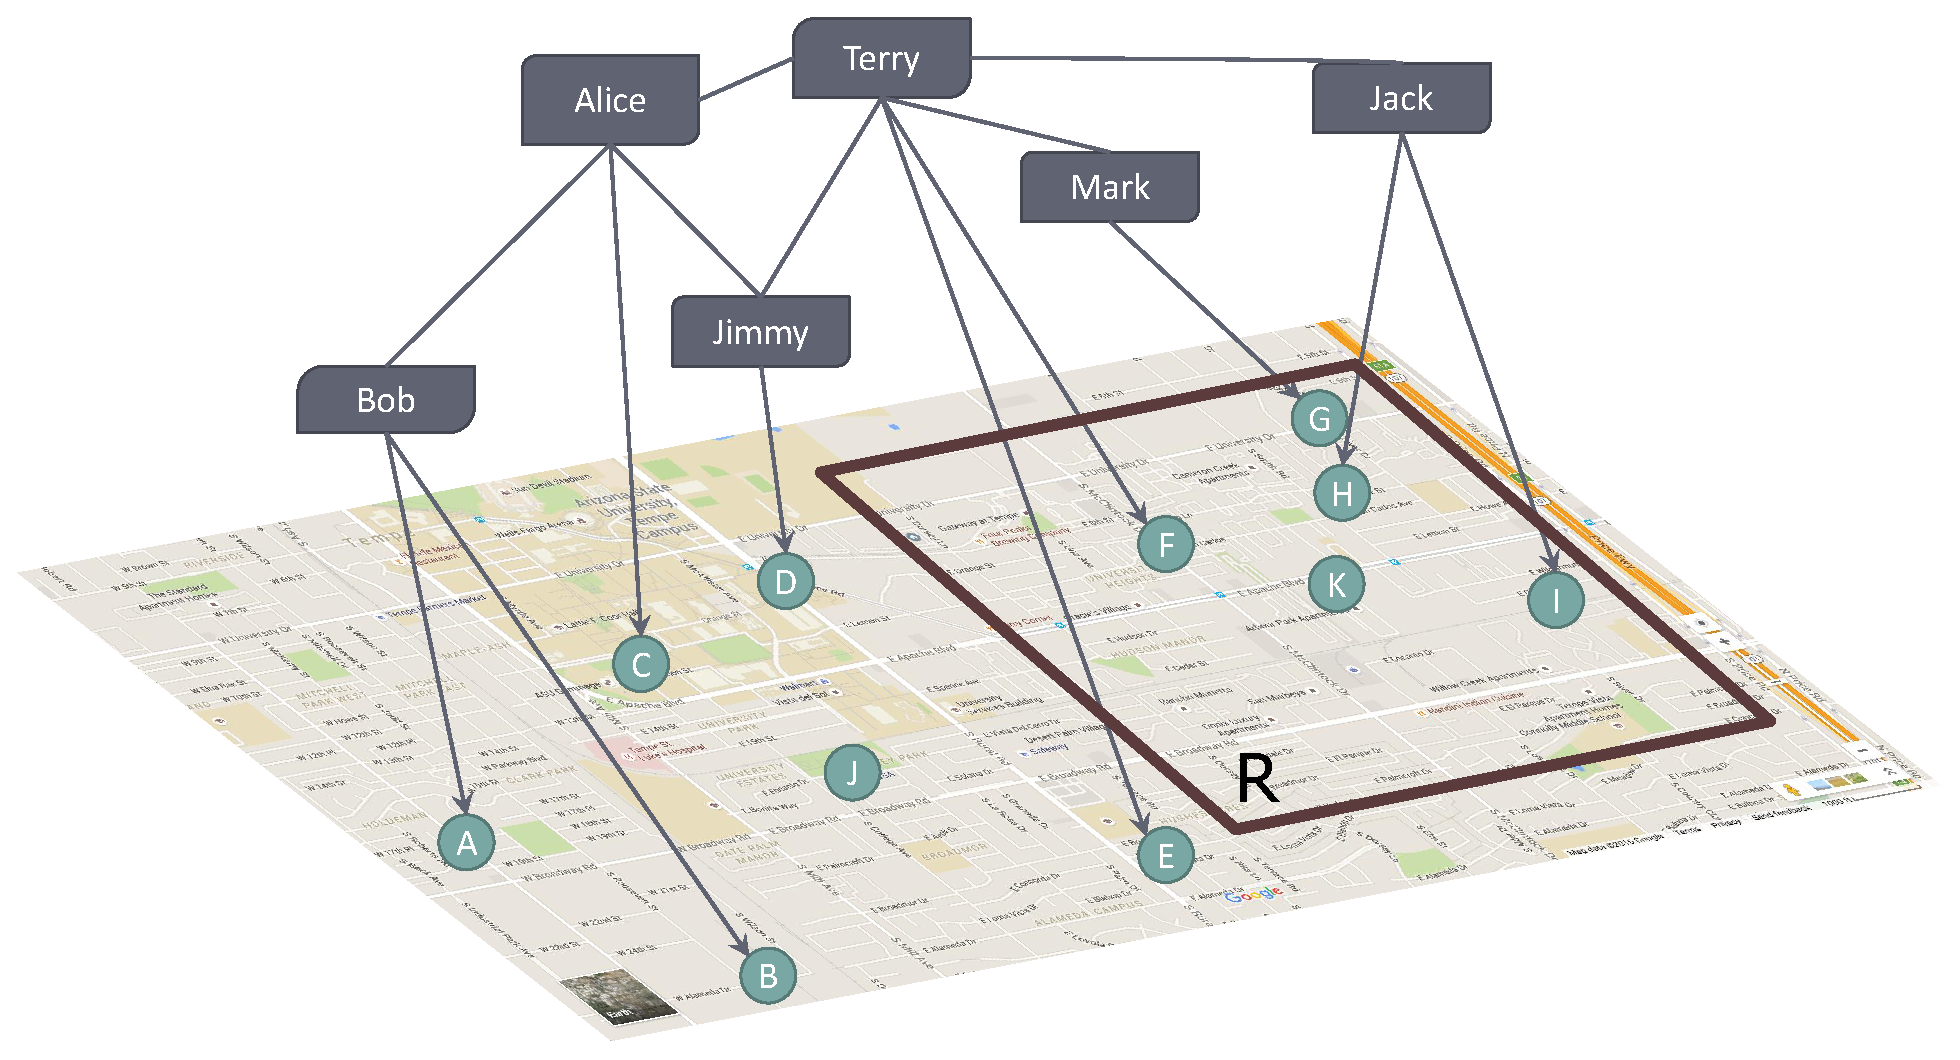
\includegraphics[width=0.88\linewidth]{images/a_motivation_example.eps}
	\caption{A motivation example}
	\label{fig:begin-example}
\end{figure}

And this paper is all about bringing these two even closer. We can predict what your best friend would have suggested to you if you wanted to go to an authentic Sushi place in SFO. Imagine restaurant recommendations from Google, are more personalized for a location instead of listing them by average user rating. To answer such queries it is required to traverse a social network and filter recommendations which fall in a given region. However minimum latency is rather imperative for such queries for the best user experience using huge social networks like Facebook, Twitter and Yelp. These graphs can be really dense, as much as, each person in the world is connected to every other person by only an average of three and a half other people!~\cite{Taa}. So the way to answer shortest path reachability queries with a spatial predicate quickly is needed even in such dense graphs (that is conditioned on a region).

Consider a restaurant recommendation system like Yelp. Every registered user can have multiple friends and also check-ins at multiple venues using this service. A small example from such a service would look like the one shown in Figure \ref{fig:begin-example} where Alice, Bob, Terry, Mark, Jack, Jimmy are people and letters from A to I are venues. Venues are also marked at the respective locations on a map. Edges between people indicate they are friends like in any social network and edges from a person to a restaurant means he/she checked-in at that location. Assume the system wants to recommend a restaurant to Bob in the marked region R and that all venues have the same average customer rating as 4.0. Any existing system would naturally return venues that fall in R in some random order as all of them are equally good. However, Bob is socially close to Terry than to Mark or Jack. Recommending restaurant F before G, H and I would make Bob happier as Terry and Bob are more similar in their tastes. Therefore, in order to provide good recommendations, we should consider both the spatial and social proximities in the search.

An easy way to solve the problem would be to find shortest distances to each venue falling in R, sorting them based on distance from the user of interest and picking the top K (whatever number is required). This disjoint approach can solve the problem but has a huge time latency especially while finding the closest vertices. Also we will be traversing huge graph aimlessly until we hit the required number of venues in R. Such a system would never be used in production. The paper~\cite{NSD2013} solves the problem in the disjoint manner using a distributed approach by implementing complex algorithms in a bottom up manner using simple distributed functions. This is a good start but we end up with other problems which distributed systems face today like network latency, consistency etc. The paper~\cite{KJY+2015} takes a new approach by combining the social and spatial constraints of the problem during the search routine but is more suited for queries like finding nodes close to a given node. However the aim is to find K closest vertices in a region from a (person) vertex in a social graph. So the big challenges ahead are to perform geosocial searches on huge graphs with (i) minimum latency, (ii) traverse the graph in a goal oriented manner towards the region unlike Dijkstra's, (iii) traverse the graph to the minimum as only the K closest vertices to a given vertex are required.

In this paper we propose a \textit{range reach paths} ({\rrp}) query which finds top-k closest vertices to a given (person) vertex in a social graph considering both the social and spatial components. Our key contributions are:
\begin{itemize}
	\item The paper studies the geosocial graph problem describing the challenge more formally and understand the need to solve this more efficiently.
	\item The paper proposes indices on social and spatial domains of the graph which form the pre-processing stage of the solution. Here graph data is stored in an organized manner to filter it based on spatial (region of interest) and social constraints (top-k closest vertices) at query time. This helps in solving the challenge of traversing to the minimum, as only best K are needed.
	\item The paper proposes a robust algorithm which uses above indices to answer top-k socio-spatial query using a modified landmark based A* algorithm by combining it with a spatial search. This solves the challenge of goal oriented search to reduce the latency even further.
	\item The paper experimentally evaluates the proposed approach with different parameter combinations on Yelp dataset. The experiments shows that our approach can achieve at least 3 times faster than existing approaches.
\end{itemize}

The rest of the paper is organized as follows: Section \ref{sec:relwork} demonstrates existing work related to {\rrp} and more insights on how our problem is different and why a better solution is required. In Section \ref{sec:preliminary} we formally define our problem in a more generic setting. Details of the proposed solution, including index structure, construction and cost analysis are given in Section \ref{sec:solution}. In Section \ref{sec:experiment} we evaluate our approach on a real dataset by comparing it with the baseline approach. Finally we conclude the paper and provide some future work in Section \ref{sec:conclusion}.
